The motivating example is about the social problem of vaccine hesitancy. This is a related problem, which got pronounced during the COVID-19 crisis, when the trust in official sources and scientific studies became a decisive factor in connection with the willingness to vaccinate \cite{petravic2021factors}. To counteract this behavior, one might imagine a predictive model based on a knowledge graph, which gives explainable recommendations to people, whether they should get vaccinated or not. Therefore, a social-themed knowledge graph about people and their COVID-19 vaccination status would be required. Due to privacy reasons, such a knowledge graph is not publicly available. However, one might expect that the introduction of electronic health records in more and more countries \cite{essen2018patient} will lead to broader availability of this kind of data to specific persons in the future. 
    
% The dataset
For the sake of comprehensibility, a tiny dataset (see figure \ref{fig:motivating_dataset}) is used for demonstration purposes. The dataset is not meant to be true in reality, but will help explain the approach (see chapter \ref{section_approach}). Each row in the table represents a type of sample, which has a weight assigned. This weight gives the proportion of this type of sample in the dataset. As described above, the example assumes a knowledge graph, which was used to extract the data. A small part of the knowledge graph is depicted in Figure \ref{fig:motivating_example_kg}. 
    
    \begin{figure}
        \centering
        \begin{tabular}{c|lclclc}
            \toprule
            weight & person & allergic\_to & gender & pregnant & country & vaccinated\\
            \midrule
            \midrule
            \(\frac{4}{12}\) & :Max & PEG & male & \(\bot\) & Germany & \(\bot\) \\
            \(\frac{1}{12}\) & :Maria & & female & \(\top\) & Germany & \(\bot\) \\
            \(\frac{6}{12}\) & :Eva   & & female & \(\bot\) & Germany & \(\top\) \\
            \(\frac{1}{12}\) & :Laura & PEG & female & \(\bot\) & Germany & \(\bot\) \\
            \bottomrule
        \end{tabular}
        \caption{Dataset about COVID-19 Vaccination}
        \label{fig:motivating_dataset}
    \end{figure}
    
    \begin{figure}
        \centering
        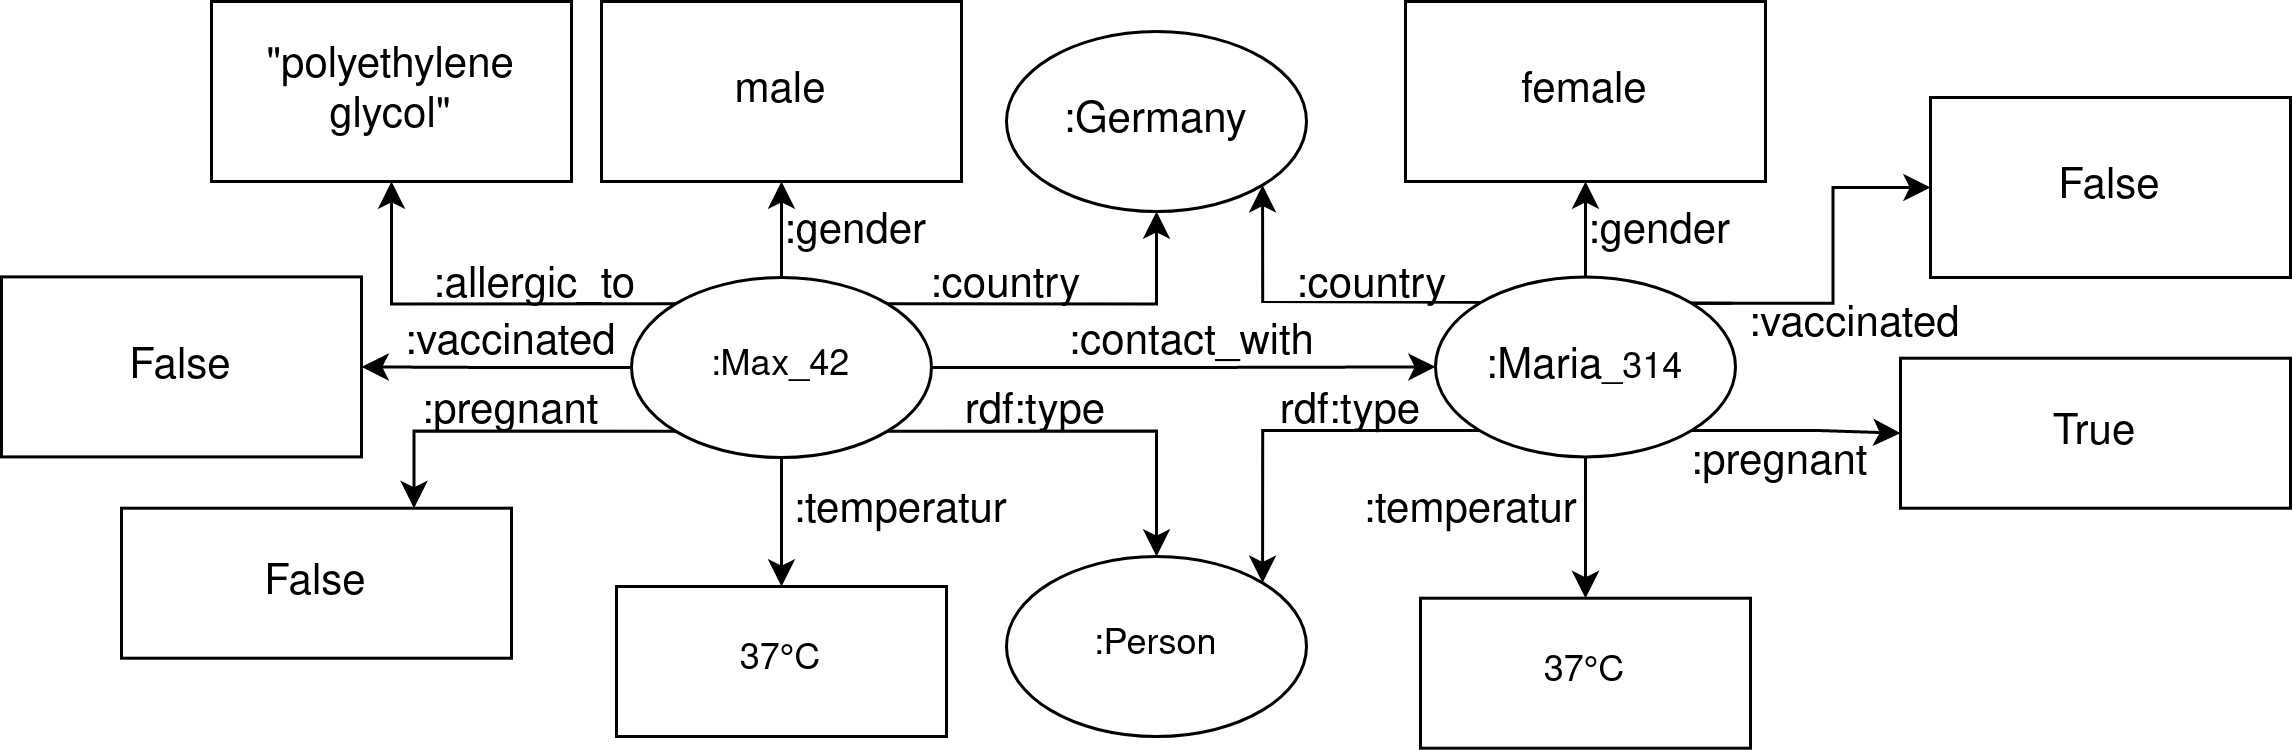
\includegraphics[width=\textwidth]{images/motivating_example/Dataset Covid-19 Part.png}
        \caption{Visualization of an RDF Graph containing some Instances of the Data}
        \label{fig:motivating_example_kg}
    \end{figure}
    
    % Knowledge Graph as Source of further insights (...this might even be the main reason, to perform constraint validation over data cleaning)   
    In this work, the goal is twofold. On the one hand, the work aims to use the additional context provided by a knowledge graph for a given set of entities. This is to be implemented to discover further insights into the patterns of machine learning models trained on the data extracted from the knowledge graph. On the other hand, a goal is to allow users to validate certain assumptions about the model using the context. To achieve that, user-defined constraints about the target of the machine learning model are validated against a knowledge graph and a model's predictions. When extracting a dataset, as in Figure \ref{fig:motivating_dataset}, from a knowledge graph, as in Figure \ref{fig:motivating_example_kg}, the graph structure of the data gets lost. In this example, there are the \uri{contact\_with} predicates, which get discarded. The example will show how this kind of semantic context, exclusively available in the knowledge graph, might be used to explain the model's predictions.
    
    % Data Quality Issues
    Available knowledge graphs suffer from data quality issues. For example, seven years ago, a paper identified certain substantial constraints over DBpedia \cite{mendes2012dbpedia}, which are frequently violated \cite{Kontokostas2014}. The situation has not changed until today \cite{valSPARQL}. This problem gets accelerated when learning from such kind of data. A model trying to generalize to this data will suffer from the same quality constraints as the data. Moreover, it will apply the recognized patterns to new data, which in turn, will also suffer from the same issues.
    
    Both, knowledge graphs as a source of further insights and data quality issues in knowledge graphs give rise to semantic constraint validation. This has the capability of identifying data points, which violate certain constraints and predictions made on the basis of these.% TODO: Somehow mention the concept of data constraints
    
    Let us assume a decision tree, trained on the given dataset, which recommends a person X, which is not allergic to PEG (included in COVID-19 vaccines) but is pregnant, not to get vaccinated (see Figure \ref{motivating_example_decision_tree}). 
    \begin{figure}
            \centering
            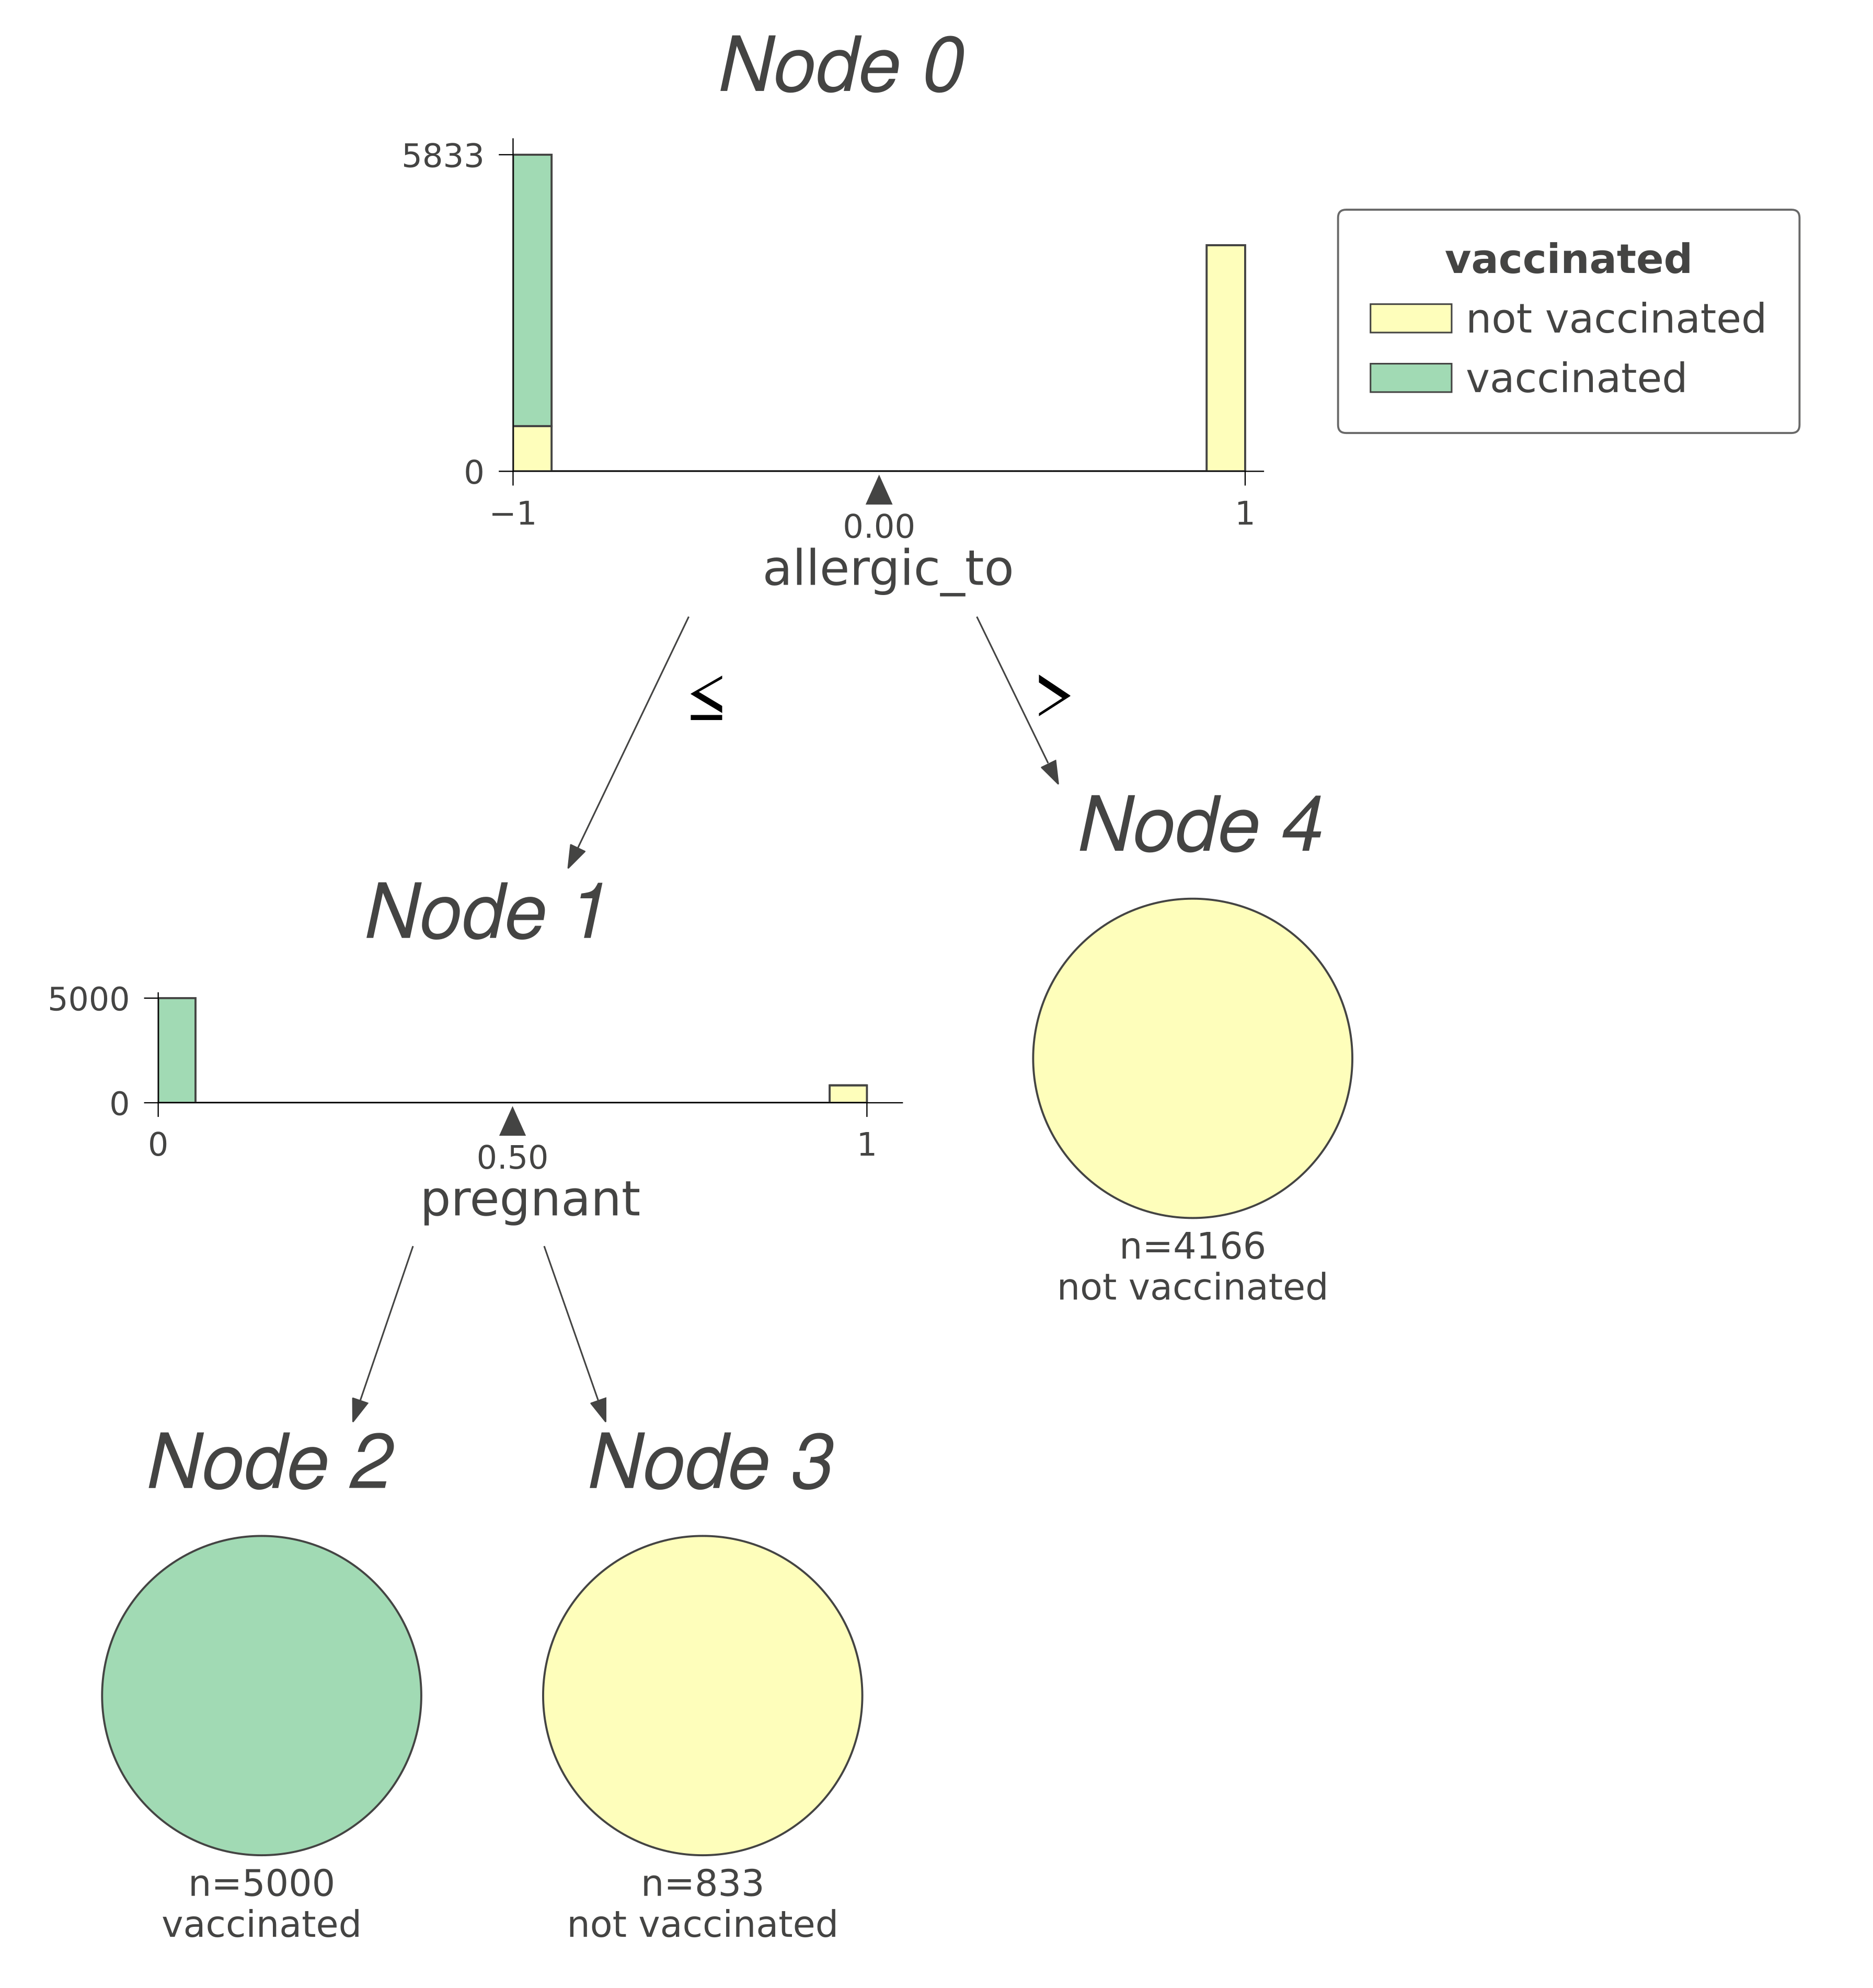
\includegraphics[width=0.6\textwidth]{images/visualizations/motivating_example_decision_tree_transparent.png}
            \caption{Decision tree trained on the dataset from figure \ref{fig:motivating_dataset} assuming $9999$ samples (n denotes the number of samples getting predictions assigned in the leaf) visualized using dtreeviz \cite{dtreeviz}}
            \label{motivating_example_decision_tree}
        \end{figure}
    \begin{figure}
            \centering
            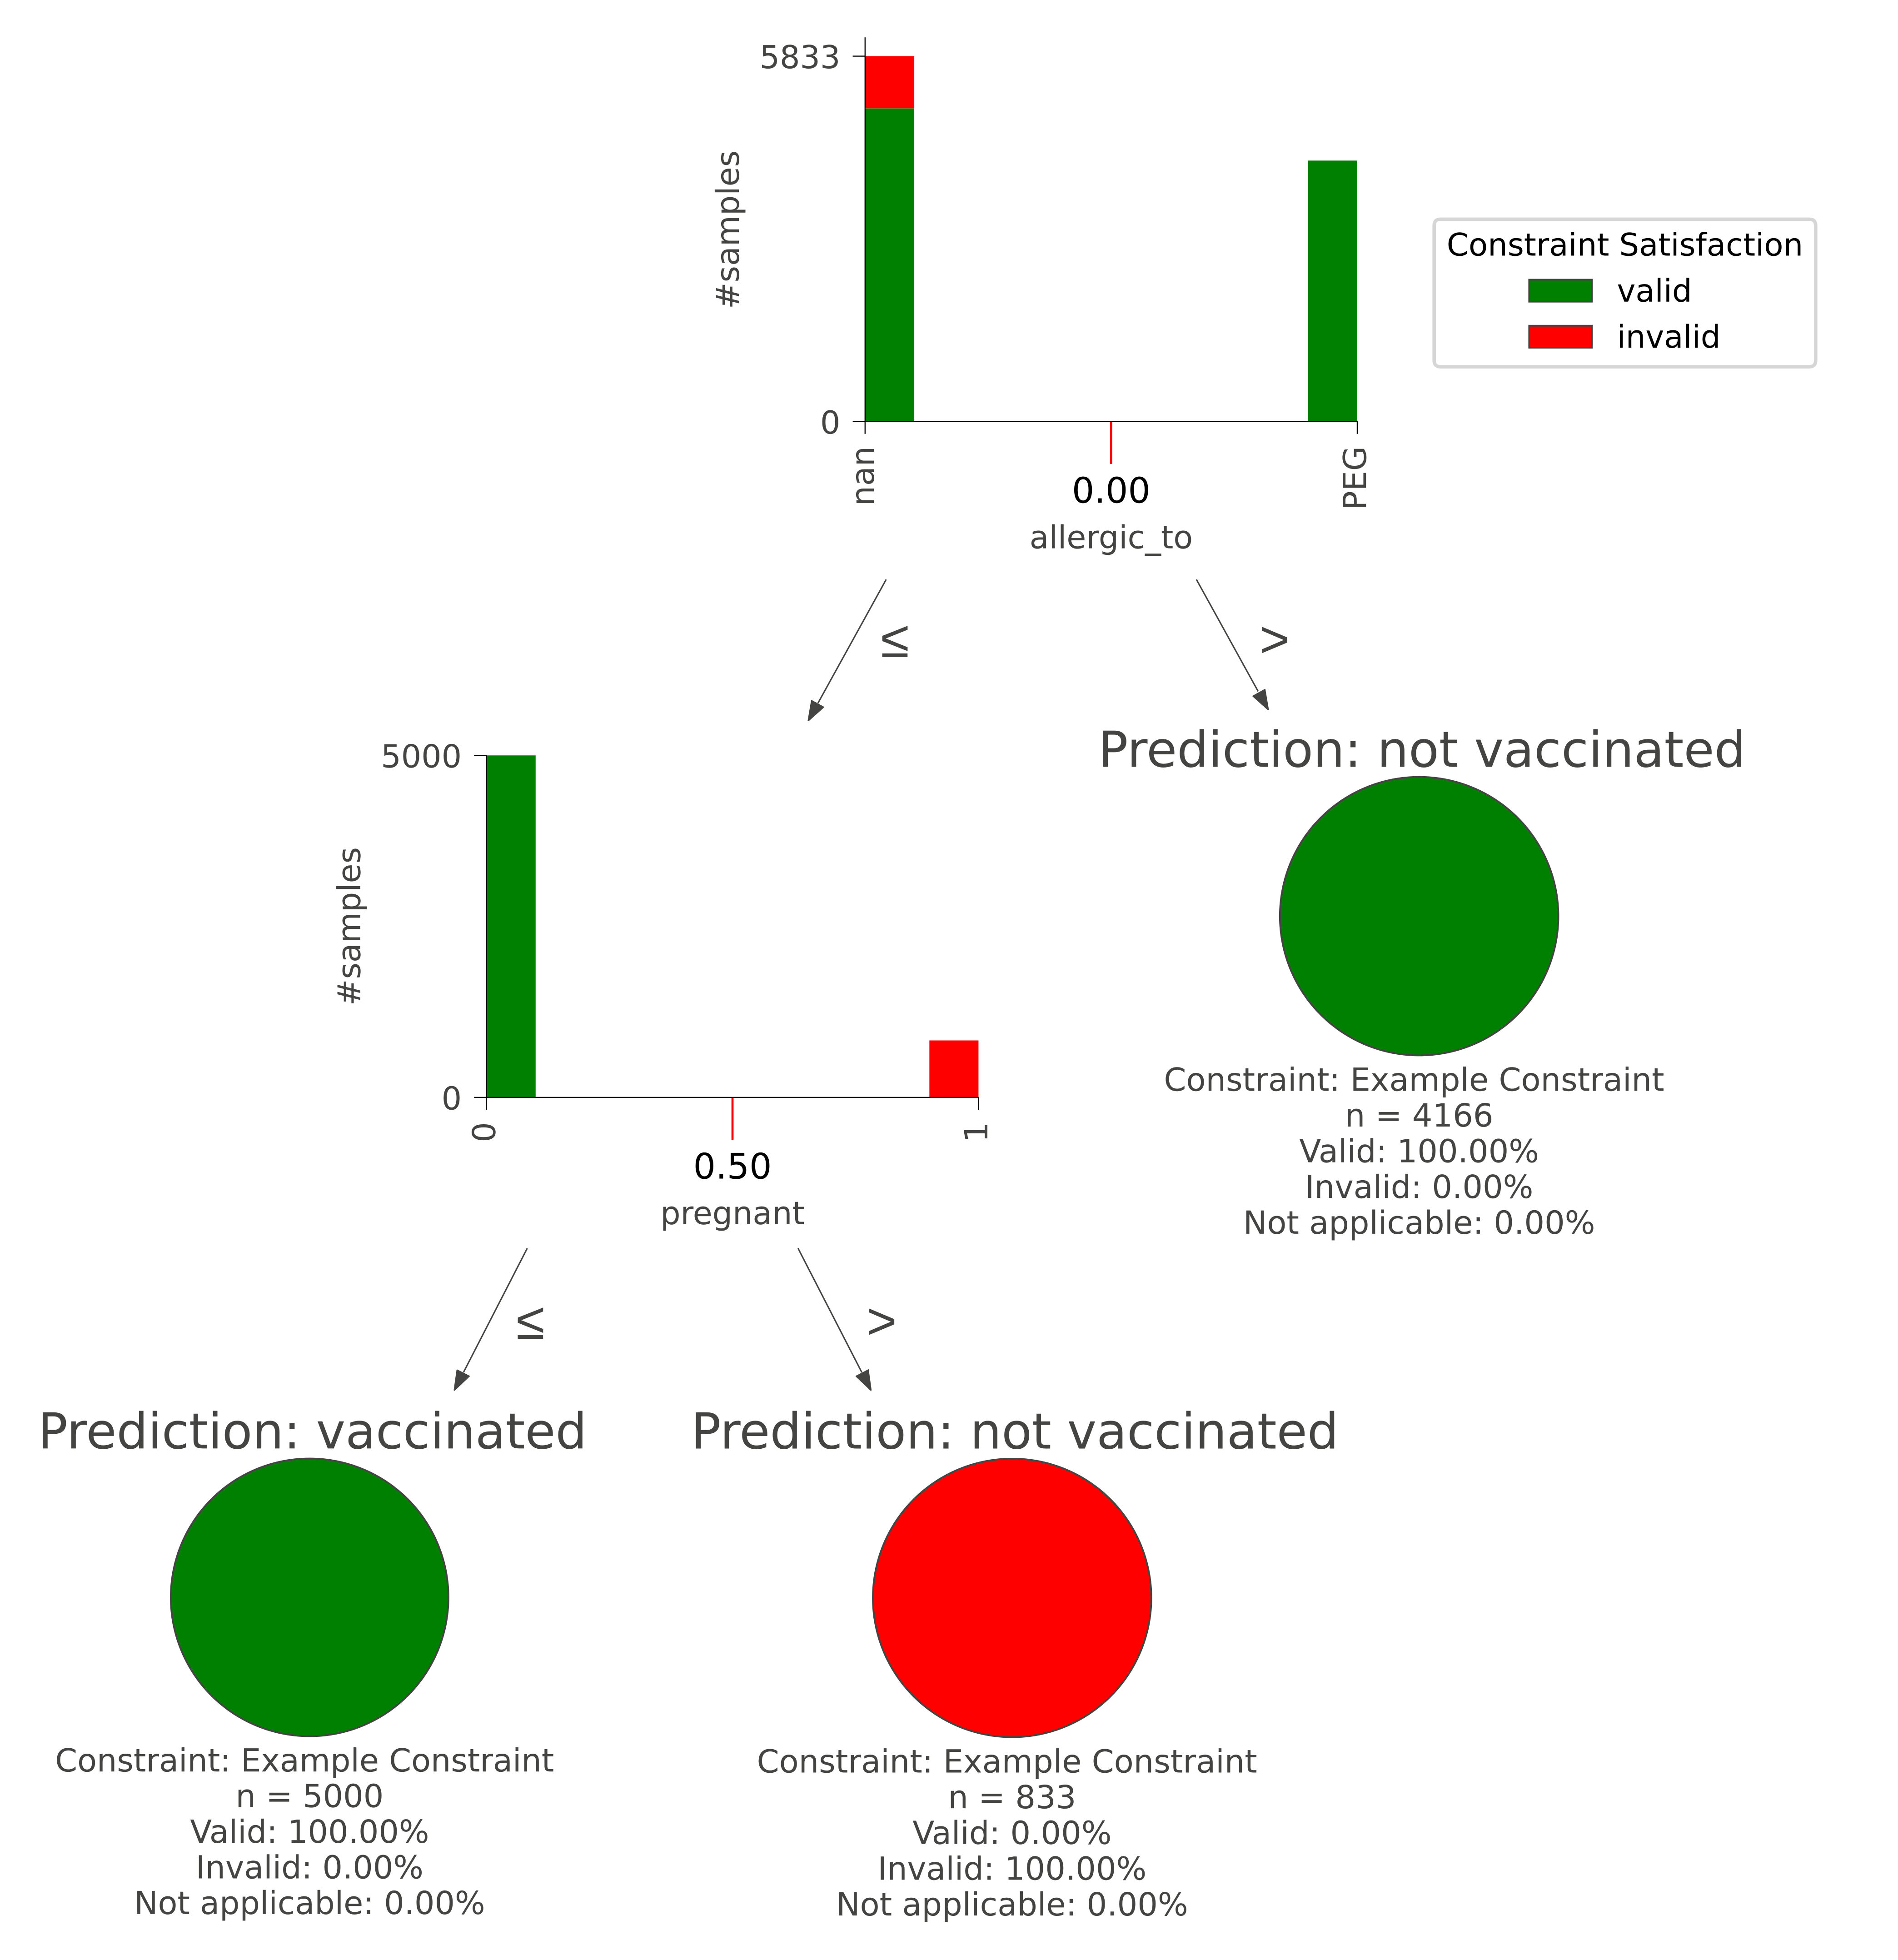
\includegraphics[width=0.6\textwidth]{images/motivating_example/Annotated Decision Tree.png}
            \caption{The decision tree of figure \ref{motivating_example_decision_tree} annotated with the validation results of the example constraint. Pregnant persons not allergic to PEG are predicted not to be vaccinated, which violates the example constraint, given the semantic context of the persons in the knowledge graph.}
            \label{motivating_example_annotated_decision_tree}
    \end{figure}
   
   Although the decision tree is already inherently explainable, and it is, therefore, known why it recommends not getting vaccinated, it remains unclear whether the decision is rational with respect to human constraints or scientific facts. For example, there might be a constraint stating: \glqq{}\emph{Every pregnant person in Germany, which has more than 20 contacts with non-vaccinated persons should get vaccinated}\grqq{}. The decision tree alone cannot be used to validate the constraint. The underlying knowledge graph is needed to count the number of contacts with vaccinated persons. An option would be to include the number of contacts with non-vaccinated persons in the dataset, but that will not guarantee that the decision tree uses this data in a constraint conform way. 
    Further, one could exclude the examples from the dataset which violate the constraint. This might be a viable approach but will only eliminate the faulty examples from the dataset, which might, in turn, lead to a better-adapted model. However, edge cases not covered by the dataset and a generalized model might continue to give predictions violating the constraint. Therefore, it might be good to learn about the model trained on the available data.
    
    As a result, the approach implicitly validates the model given a set of constraints and the knowledge graph to explain the model's prediction with respect to the constraints. In this context, ``implicitly'' means that each sample in the dataset is used to conclude the model's behavior. This kind of information is then used to visualize constraint satisfaction. An example of such a visualization is shown in Figure \ref{motivating_example_annotated_decision_tree}, which demonstrates that the prediction the model makes for person X violates the constraint. On the other hand, it confirms the other predictions of the model. For example, the model suggests not getting vaccinated if someone is allergic to PEG. The constraint does not contradict these predictions. Therefore, a potential user of the model can be sure that the model's decision is not made based on data for which the model makes invalid predictions.
        
    Performing constraint validation this way has further advantages: One might find errors in the model, which need to be solved, or reject invalid predictions. Furthermore, a model can be checked to apply in a different environment with different constraints.

    
    
    
    
    
    %\begin{figure}
    %    \centering
    %    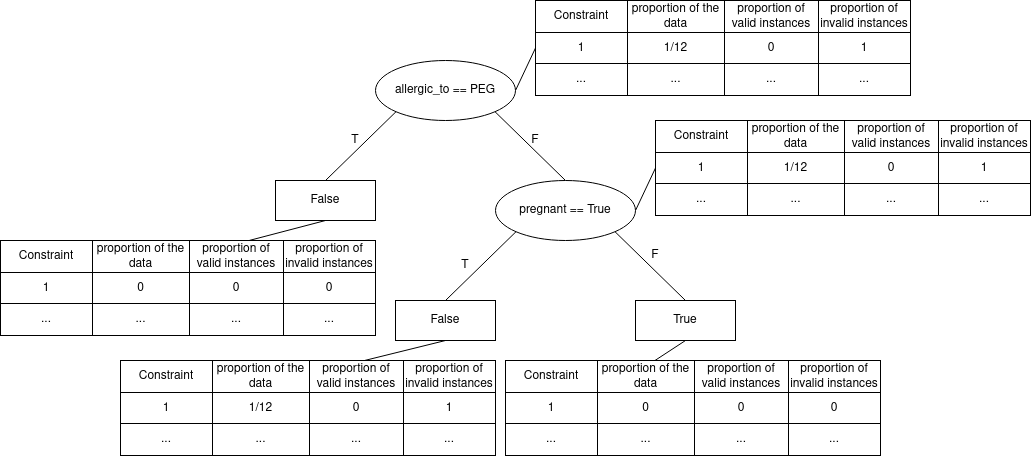
\includegraphics[width=\textwidth]{images/motivating_example/Annotated Decision Tree.drawio.png}
    %    \caption{Annotated Decision Tree}
    %    \label{motivating_example_annotated_decision_tree}
    %\end{figure}
    
    % Description of a possible result tree
    % Figure \ref{motivating_example_annotated_decision_tree} shows such a tree. The process of creating the decision tree is described in section \ref{decision_tree_algorithm}. For each splitting node and leaf (which contains the decision whether on should get vaccinated) in the tree there is a table with annotation, which gives for each constraint the proportion of the whole data, to which the constraint applies and also the proportion of valid and invalid instances, identified in this proportion of the data.
    
    % An example constraint proposed
    % There might be multiple constraints as denoted by the dots in the annotations of the decision tree. But here only one constraint is defined, which is referred to as constraint 1: \glqq{}\emph{Every pregnant person in Germany, which has more than 20 contacts should get vaccinated}\grqq{}. The constraint can clearly be expressed in the form of an implication having a set of conditions on the training instance found in the knowledge graph on the left hand side and the target on the right hand side.
    %\begin{gather}
    %            S \implies (\text{vaccinated} = \top) \label{motivating_example_constraint}
    %\end{gather}

    % Following the W3C recommendation $S$ should be expressed as SHACL Shape Network \cite{knublauch2017shapes}. This has the already mentioned advantage that it allows to use information encoded in the knowledge graph. The one for constraint $1$ can be found in listing \ref{lst:motivating_example_shape_network}. 
    
    %\lstset{language=html}
    %\begin{lstlisting}[captionpos=b, caption=S in case of Constraint 1, label=lst:motivating_example_shape_network, basicstyle=\ttfamily, frame=single]
    %@prefix : <http://example.org/>
    %@prefix sh : <http://www.w3.org/ns/shacl#>
    %:PersonShape
    %    a sh:NodeShape ;
    %    sh:targetClass :Person ;
    %    sh:property [
    %        sh:path :pregnant ;
    %        sh:minCount 1 ;
    %        sh:hasValue True .
    %    ] ;
    %    sh:property [
    %        sh:path :country ;
    %        sh:minCount 1 ;
    %        sh:hasValue "Germany" .
    %    ] ;
    %    sh:property [
    %        sh:path :contact_with;
    %        sh:minCount 20 .
    %    ] .
    %\end{lstlisting}
    
    % Now one would have to make use of the full knowledge graph during training and a validation process to create the annotations provided in figure \ref{motivating_example_annotated_decision_tree}. But inspection of the dataset in figure \ref{motivating_dataset} and additional statistics about the number of contacts per person in figure \ref{motivating_example_statistics} allows the given annotation to be performed by hand. Only the persons marked as \url{:Maria} conform to $S$.
    % According to the dataset in figure \ref{motivating_dataset} \url{:Maria} makes up $\frac{1}{12}$ of the total dataset. 
    
    
    % Therefore following the decision path in figure \ref{motivating_example_annotated_decision_tree} corresponding to \url{:Maria} shows that all the annotations referring to the proportion of the data, which conforms to constraint $1$ are set to $\frac{1}{12}$. The decision path leads to the prediction that \url{:Maria} should not get vaccinated. But that violates the constraint given in formula \ref{motivating_example_constraint}. Finally this result is propagated back up in the decision tree, such that for each node the proportion of invalid instances given the data which conforms to $S$ is set to $1$. 
    
    % \begin{figure}
    %    \centering
    %    \begin{tabular}{l|l}
    %         \toprule
    %         person & \#contact\_with \\
    %         \midrule
    %         \midrule
    %         :Max &  $15$\\
    %         :Maria & $25$\\
    %         :Eva & $30$\\
    %         :Laura & $10$\\
    %         \bottomrule
    %    \end{tabular}
    %    \caption{Statistics regarding contact\_with}
    %    \label{motivating_example_statistics}
    %\end{figure}